\documentclass[12pt,fleqn]{article}
\usepackage{../lecture-notes/vkCourseML}
\usepackage{lipsum}
\usepackage{indentfirst}
\usepackage{graphicx}
\graphicspath{{./figures/}}
\usepackage{tikz}
\usetikzlibrary{positioning,arrows}
\usepackage{amsmath}
\title{Машинное обучение, ФКН ВШЭ\\Семинар №9}
\date{}
\author{}
\begin{document}
\maketitle


\section{Градиентный бустинг}

На лекциях обсуждался градиентный бустинг~--- один из самых мощных
методов в машинном обучении.
Он позволяет воспользоваться выразительной силой решающих деревьев и при этом
контролировать их переобучение.
Ниже мы пройдём по основным блокам градиентного бустинга
и поймём, почему они устроены именно так.

Для начала вспомним основные принципы градиентного бустинга.
Будем искать алгоритм, оптимизирующий некоторую дифференцируемую функцию потерь $L(y, z)$, в виде взвешенной суммы базовых алгоритмов:
\[
    a_N(x)
    =
    \sum_{n = 0}^{N}
        \gamma_n b_n(x).
\]
Как правило, веса~$\gamma_n$ не подбираются и полагаются равными единице~(поскольку, как правило, в деревьях всё равно потом тщательно подбираются прогнозы в листьях),
но пока будет рассматривать общий случай.

Идея бустинга заключается в последовательном построении алгоритмов, каждый из которых учитывает ошибки построенной до сих пор композиции:
\[
    \sum_{i = 1}^{\ell}
        L(y_i, a_{N - 1}(x_i) + \gamma_N b_N(x_i))
    \to
    \min_{b_N, \gamma_N}
\]

После выбора каких-нибудь простых~$\gamma_0$ и $b_0(x)$~(например, для задачи регрессии
можно положить~$\gamma_0 = 1$ и $b_0(x) = \frac 1\ell \sum_{i=1}^\ell y_i$)
все последующие базовые алгоритмы стараются приблизить антиградиент функционала ошибки, взятый в точках $z = a_{N - 1}(x_i)$:
\[
    s_i
    =
    -
    \left.
    \frac{\partial L(y_i, z)}{\partial z}
    \right|_{z = a_{N - 1}(x_i)}
\]

При этом приближается антиградиент с точки зрения квадратичной функции потерь:
\[
    b_N(x)
    =
    \argmin_{b \in \AA}
        \sum_{i = 1}^{\ell}
            \left(
                b(x_i) - s_i
            \right)^2
\]

Подбор коэффициентов производится просто через задачу одномерной оптимизации:
\[
    \gamma_N
    =
    \argmin_{\gamma \in \mathbb{R}}
    \sum_{i=1}^{\ell}
    L(y_i, a_{N-1}(x_i) + \gamma b_N (x_i))
\]

Обсудим теперь подробнее некоторые моменты.

\subsection{Почему градиентный бустинг устроен именно так?}

\paragraph{Зачем сдвиги в бустинге считаются через производные функции потерь?}
Почему нельзя использовать сдвиги вида~$y_i - a_{N - 1}(x_i)$?
Казалось бы, если удастся хорошо приблизить эти отклонения с помощью~$b_N(x)$,
то будет выполнено~$a_{N-1}(x_i) + b_N(x_i) \approx y_i$.

Мы решаем сложные задачи, в которых, скорее всего, ещё и не идеальные данные,
есть шумы, выбросы и так далее.
Это означает, что не стоит рассчитывать на получение непереобученной модели
с нулевой ошибкой на обучающей выборке.
Мы это понимаем, и поэтому через функцию потерь определяем,
какие ошибки более приемлемы, чем другие.
Если использовать сдвиги, равные разности правильного ответа и прогноза текущей композиции,
то мы полностью игнорируем эти требования.
Разберём несколько примеров.

Начнём с регрессии.
Допустим, у нас несимметричная функция потерь, где мы сильнее штрафуем за завышение прогноза:
\begin{equation}
\label{eq:asymmetricLoss}
    L(y, z)
    =
    \frac{1}{2}
    (10 [z \geq y] + [z < y])
    (y - z)^2.
\end{equation}
Рассмотрим два объекта~$x_1$ и~$x_2$ с правильными ответами~$y_1 = y_2 = 0$
и прогнозами текущей композиции~$a_{N - 1}(x_1) = 5$ и~$a_{N - 1}(x_2) = -5$.
Если взять сдвиги, равные~$y_i - a_{N - 1}(x_i)$,
то базовая модель будет пытаться одинаково скорректировать прогнозы на обоих объектах.
Но, конечно, надо сильнее сконцентрироваться на коррекции прогноза на первом объекте,
поскольку на нём штраф больше: $L(0, 5) = 125 > 12.5 = L(0, -5)$.
Сдвиги, посчитанные через частные производные, лучше отражают приоритеты:~$s_1 = -50$, $s_2 = 5$.
При этом не страшно, что на первом объекте мы сделаем слишком большую корректировку~---
это будет исправлено с помощью веса~$\gamma_N$ базовой модели или с помощью других техник.

Обсудим теперь обучение на абсолютную ошибку~$L(y, z) = |y - z|$.
Вычислим для неё сдвиги:
\[
    s_i = - \left. \frac{\partial |y_i - z|}{\partial 
        z} \right|_{z=a_{N-1}(x_i)} = 
    \Bigl. \sign(y_i - z) \Bigr|_{z=a_{N-1}(x_i)} =
    \sign(y_i - a_{N-1}(x_i))
\]
И это снова более логично, чем обучение на~$y_i - a_{N - 1}(x_i)$!
Мы знаем, что с точки зрения квадратичной ошибки даже небольшое уменьшение серьёзной ошибки
оказывается лучше, чем доведение небольшой ошибки до нуля:
\begin{align*}
    &L(0, 1000) - L(0, 999) = 1999 > 1 = L(0, 1) - L(0, 0).
\end{align*}
Поэтому для квадратичной ошибки разумно использовать сдвиги~$y_i - a_{N - 1}(x_i)$,
поскольку чем больше отклонение от правильного ответа, тем больше штраф и тем сильнее надо корректировать прогнозы.
У абсолютной ошибки такого свойства нет, изменения штрафа не зависят от отклонения прогноза от факта.
Поэтому независимо от того, на каком объекте мы приблизим прогноз к правильному ответу на единицу,
средняя абсолютная ошибка улучшится на одну и ту же величину.
У нас как раз получилось, что сдвиги на всех объектах одинаковы по модулю и отличаются лишь знаком~---
это соответствует описанному выше свойству абсолютной ошибки.

Перейдём к классификации.
Если у нас два класса~($\mathbb{Y} = \{-1, +1\}$),
и сама композиция также возвращает прогноз из~$\mathbb{Y}$,
то отклонения всегда будут принимать значения из небольшого множества:
$|y_i - a_{N - 1}(x_i)| \in \{0, +2\}$.
Получается, что если модель уже выдаёт правильный ответ, то сдвиги будут равню нулю,
и никакие модификации для этого объекта вноситься не будут.
Разумеется, это нас не устраивает~--- как правило, функции потерь в классификации
стараются максимизировать отступ (или хотя бы довести его до определённого положительного значения),
а полученные нами сдвиги никак не зависят от отступа.

Чтобы это исправить, договоримся, что наша композиция~$a_N(x)$ будет выдавать вещественные числа,
и по смыслу они будут являться оценками~\emph{логита},
то есть логарифма отношения вероятности положительного класса к вероятности отрицательного класса:
\[
    a_N(x)
    =
    \log
    \frac{
        p(y = +1 \cond x)
    }{
        1 - p(y = +1 \cond x)
    }
\]
Если выразить отсюда вероятность, то получится
\[
    p(y = +1 \cond x)
    =
    \sigma\left(
        a_N(x)
    \right)
    =
    \frac{
        1
    }{
        1 + \exp(-a_{N}(x))
    }
\]
То есть сигмоида от модели будет оценивать вероятность положительного класса.
Эту же идею мы использовали при обучении линейных классификаторов~--- там скалярное произведение как раз
оценивало логиты.
С таким подходом обучение на~$y_i - a_{N - 1}(x_i)$ выглядит ещё менее логичным, поскольку в этом случае
мы будем пытаться уменьшить отступ там, где он большой положительный,
то есть по сути будем запрещать модели быть уверенной в своём ответе.

В завершение посчитаем сдвиги для логистической функции потерь:
$L(y, z) = \log (1 + \exp(-yz))$.
Для этого вспомним, что логистическая функция потерь выражается через сигмоиду $\sigma(x) 
= \frac{1}{1 + \exp(-x)}$ следующим образом:
\[
    L(y, z) = \log \left( \frac{1}{\sigma(yz)} \right) = -\log \sigma(yz)
\]
Далее, пользуясь формулой для производной сигмоиды $\sigma'(x) = \sigma(x)(1 - \sigma(x))$,
получаем
\begin{align*}
    s_i &= \left. \frac{\partial \log \sigma(y_i z)}{\partial z} 
        \right|_{z=a_{N-1}(x_i)} =
    \left. \frac{1}{\sigma(y_i z)} \sigma(y_i z) (1 - \sigma(y_i z)) y_i
        \right|_{z=a_{N-1}(x_i)} =\\
    &= (1-\sigma(y_i a_{N-1}(x_i))) y_i =
    \frac{y_i}{1 + \exp(y_i a_{N-1}(x_i))}.
\end{align*}
Заметим, что чем больше отступ, тем меньше будут сдвиги по модулю.

\paragraph{Почему базовая модель приближает сдвиги по MSE, а не по исходной функции потерь?}
Казалось бы, надо везде, где можно, использовать исходную функцию потерь,
в том числе и для обучения базовой модели:
\[
    \sum_{i = 1}^{\ell}
        L(s_i, b_N(x_i))
    \to
    \min_{b_N}
\]

Функция потерь задаёт штрафы для прогнозов моделей.
При этом сдвиги~$s_i$ уже содержат в себе информацию о том, в какую сторону и как сильно
надо корректировать прогнозы композиции, и будет разумно аппроксимировать их
с одинаковой важностью для всех объектов.
Если же и здесь использовать исходную функцию потерь, то иногда можно
получить странные эффекты.

Вернёмся к несимметричной функции потерь~\eqref{eq:asymmetricLoss}.
У нас было два объекта с правильными ответами~$y_1 = y_2 = 0$,
прогнозами текущей композиции~$a_{N - 1}(x_1) = 5$ и~$a_{N - 1}(x_2) = -5$
и сдвигами~$s_1 = -50$, $s_2 = 5$.
Наша функция потерь будет сильнее поощрять алгоритмы,
которые выдадут на первом объекте корректировку сильнее~$-50$,
а на втором объекте~--- до~$5$.
Но это не имеет никакого смысла, поскольку дерево лишь должно выучить, уменьшаем или увеличиваем мы
выход композиции на каждом объекте, и изменение на первом объекте должно быть больше относительно изменения
на втором объекте.

В случае с классификацией всё ещё хуже.
Например, если мы работаем с логистической функцией потерь, то
при обучении одной модели на классы она имеет смысл правдоподобия,
а также заставляет модель корректно оценивать вероятности классов.
Если же в неё вместо правильных классов подставить сдвиги, то оптимизационную задачу
будет достаточно сложно проинтерпретировать.

Заметим, что в то же время существуют способы сильнее учитывать исходную функцию потерь
в процессе обучения базовых моделей~--- мы разберём их, когда будем обсуждать XGBoost и связанные с ним
модификации классического алгоритма.

Отметим также, что минимизация MSE имеет смысл в бустинге по ещё одной причине.
Распишем этот функционал:
\[
    \sum_{i = 1}^{\ell}
        (b_N(x_i) - s_i)^2
    =
    \sum_{i = 1}^{\ell}
        (b_N^2(x_i)
        -
        2 s_i b_N(x_i)
        +
        s_i^2).
\]
Последнее слагаемое не зависит от модели и поэтому никак не повлияет на решение оптимизационной задачи.
Остаются два слагаемых:
\[
    \sum_{i = 1}^{\ell}
        (b_N^2(x_i)
        -
        2 s_i b_N(x_i))
    =
    \sum_{i = 1}^{\ell}
        b_N^2(x_i)
    -
    2
    \|s\|
    \|b_N(x)\|
    \cos(s, b_N(x))
    \to
    \min_{b_N},
\]
где~$\|s\| = \sqrt{\sum_{i = 1}^{\ell} s_i^2}$,
$\|b_N(x)\| = \sqrt{\sum_{i = 1}^{\ell} b_N^2(x_i)}$,
$\cos(s, b_N(x))$~--- косинус угла между соответствующими векторами.
Получается, что мы (с некоторыми оговорками) требуем от модели, чтобы она угадала направление
корректировки прогнозов на всей обучающей выборке.

\paragraph{Почему нельзя просто обучить одно глубокое решающее дерево?}
Понятно, что если делать это неаккуратно, то дерево переобучится, но наверняка ведь можно
контролировать это?

Действительно, так можно делать. Но как контролировать переобучение?
Можно ограничить глубину дерева или минимальное число объектов в листе, но это слишком просто~---
не факт, что эти критерии гарантируют хороший результат на тестовой выборке.
Это означает, что во время построения надо контролировать ошибку на тесте,
и с учётом неё принимать решение об остановке построения дерева в каждой вершине.
Более того, из-за жадной природы алгоритм построения дерева может выбирать некорректные
разбиения в начале~--- если мы поймём, что именно из-за них случается переобучение, может
потребовать радикально перестраивать дерево.
В итоге получится громоздкий и трудоёмкий алгоритм.

Бустинг же позволяет балансировать между сложностью и качеством итоговой модели.
На каждом шаге он строит очень небольшие деревья, которые не могут привести к сильной подгонке под
обучающую выборку.
При этом после добавления каждого дерева, как правило, проверяется ошибка на тестовых данных,
и если начинается переобучение, то процедура построения композиции прекращается.

\paragraph{Можно ли задействовать идеи из модификаций градиентного спуска?}
Да, можно!
Дальше в курсе мы разберём, как можно задействовать вторые производные
функции потерь для имитации оптимизации второго порядка.
Но также можно использовать и другие подходы~--- например, из метода инерции.

В работе~\cite{lu20accelerating} предлагается адаптировать ускоренный метод инерции Нестерова~(Nesterov momentum).
Разберём сначала этот метод.
Напомним, что обычный метод инерции устроен так:
\begin{align*}
    &h_0 = 0;\\
    &h_k = \alpha h_{k - 1} + \eta_k \nabla_w Q(w^{(k-1)});\\
    &w^{(k)} = w^{(k-1)} - h_k.
\end{align*}
Заметим, что мы ещё до вычисления~$h_k$ знаем, что сдвинемся в направлении~$h_{k - 1}$,
немного скорректированном на антиградиент функционала ошибки в точке~$w^{(k-1)}$.
Воспользуемся этим наблюдением и сначала сдвинемся по~$h_{k - 1}$,
а затем вычислим антиградиент уже в этой точке и шагнём по нему:
\begin{align*}
    &h_0 = 0;\\
    &h_k = \alpha h_{k - 1} + \eta_k \nabla_w Q(w^{(k-1)} - \alpha h_{k - 1});\\
    &w^{(k)} = w^{(k-1)} - h_k.
\end{align*}

Теперь перенесём этот метод на градиентный бустинг.
Помимо самой композиции~$a_{N}(x)$ будем теперь строить <<инерционную>> модель~$h_N(x)$,
которая будет как бы накапливать антиградиенты.
В начале инициализируем её так же, как и саму композицию:~$h_0(x) = a_0(x) = b_0(x)$.
Допустим, мы сделали~$N - 1$ шаг градиентного бустинга и построили~$a_{N - 1}(x)$ и~$h_{N - 1}(x)$.
Базовая модель~$b_N(x)$ должна аппроксимировать антиградиент~--- значит, теперь будем обучать её
на сдвиги вида
\[
    s_i
    =
    -
    \left.
    \frac{\partial L(y_i, z)}{\partial z}
    \right|_{z = a_{N - 1}(x_i) + \alpha h_{N - 1}(x_i)}
\]
Видно, что здесь в качестве обучаемых параметров у нас выступают выходы уже построенной композиции~$a_{N - 1}(x_i)$,
а в качестве инерции~--- выходы функции~$h_{N - 1}(x_i)$.
Теперь мы можем обновить инерционную функцию и саму композицию:
\begin{align*}
    &h_N(x)
    =
    \alpha h_{N - 1}(x)
    +
    \eta
    b_N(x);\\
    &a_N(x)
    =
    a_{N - 1}(x)
    +
    h_N(x).
\end{align*}
В статье используется немного модифицированная версия, где параметр~$\alpha$
меняется в зависимости от номера итерации и влияет также на длину шага~$\eta$.
Помимо этого отмечается, что указанные формулы работают не лучшим образом,
поскольку в инерционной функции накапливается ошибка, связанная с неточным
приближением антиградиента базовыми функциями.
Это исправляется усложнённой процедурой построения инерционной функции~---
но это детали, а главное, что идеи из оптимизация действительно удаётся
перенести и на градиентный бустинг, что открывает большой простор для улучшений.

\paragraph{Если градиентный бустинг такой мощный, то зачем нужны другие модели?}
Прежде всего, бустинг может не очень хорошо работать на малых выборках и в случаях,
когда признаков очень много.
Но есть ещё один нюанс~--- бустинг над деревьями не умеет экстраполировать.
Рассмотрим пример.

\begin{figure}[t]
  \begin{multicols}{2}
    \hfill
    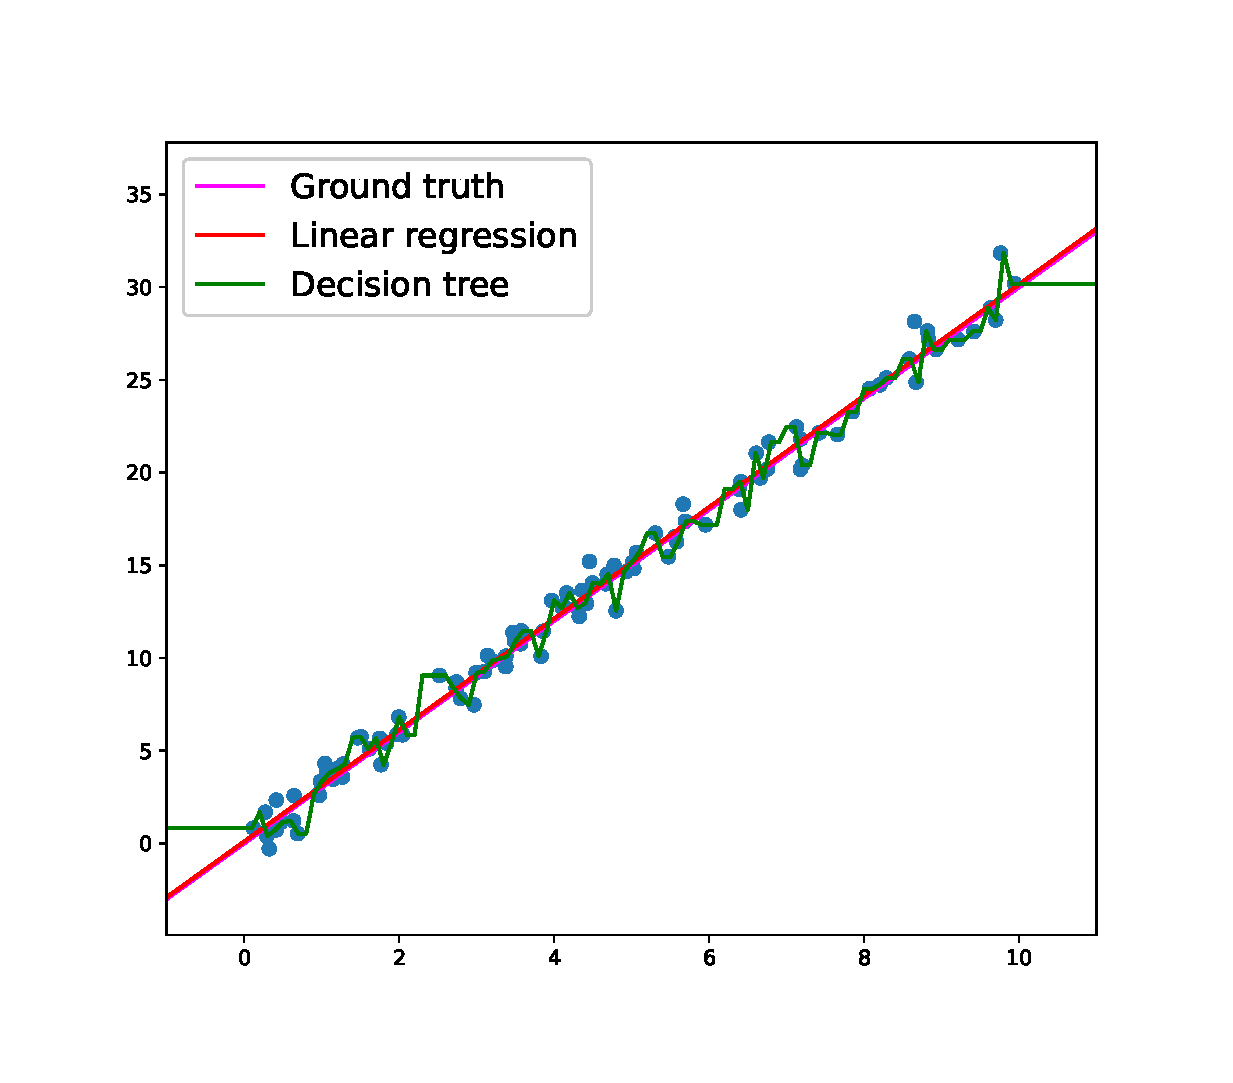
\includegraphics[width=80mm]{img/extrapolation-1.eps}
    \hfill
    \caption{Прогнозы моделей на обучении.}
    \label{fig:extr1}
    \hfill
    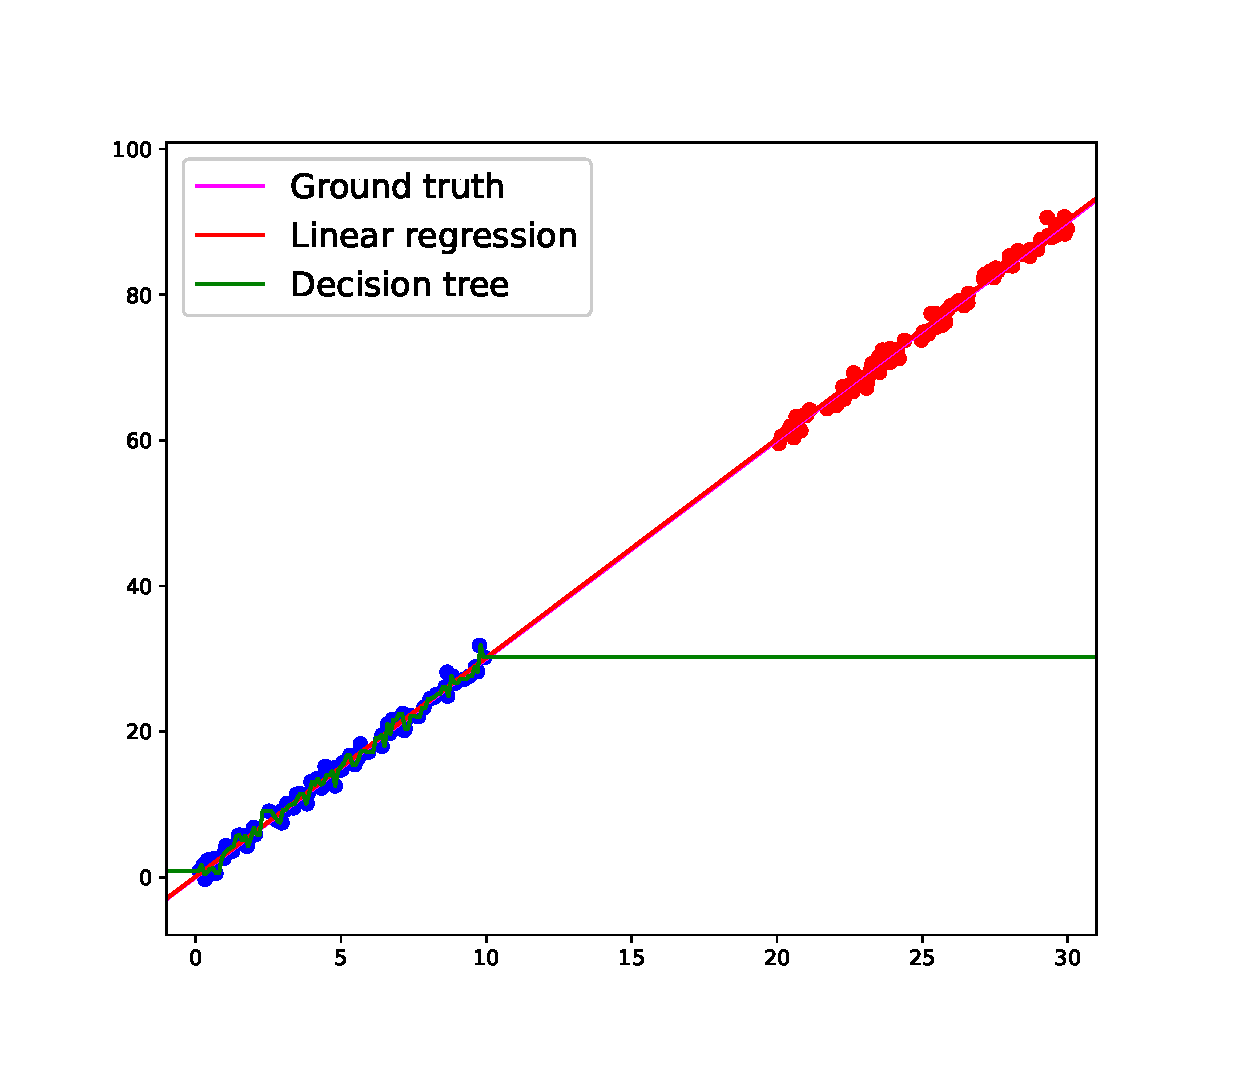
\includegraphics[width=80mm]{img/extrapolation-2.eps}
    \hfill
    \caption{Прогнозы моделей на полных данных.}
    \label{fig:extr2}
  \end{multicols}
\end{figure}

Пусть объекты описываются одним признаком, а зависимость между этим признаком
и целевой переменной действительно линейная:
$y(x) = a x + \varepsilon$, $\varepsilon \sim \mathcal{N}(0, \sigma^2)$.
В обучающей выборке признак принимает значения из отрезка~$[0, 10]$.
Обучим линейную модель и решающее дерево, результат показан на рис.~\ref{fig:extr1}.

Вполне может оказаться, что на новых данных закономерность будет такой же, но при этом
признаки будут принимать значения, не встречавшиеся на обучающей выборке.
Например, в нашем случае новые данные могут иметь значения признака из отрезка~$[20, 30]$.
Поведение моделей показано на рис.~\ref{fig:extr2}.
Видно, что деревья плохо подходят для экстраполяции.
При этом ситуация с изменением распределения признаков вполне может встретиться на практике,
и это иногда решается как раз с помощью комбинирования линейных моделей и градиентного бустинга~(который
обучается для корректировки прогнозов линейной модели).

\subsection{Сложность обучения бустинга}

Чтобы закрепить понимание градиентного бустинга, посчитаем сложность обучения и применения для него.

\begin{vkProblem}
Дана выборка из $\ell$ объектов, описываемых $d$ признаками. Приведите временную асимптотику обучения и построения прогнозов для композиции вида $a_N(x) = \sum_{n=0}^N b_n(x)$ над решающими деревьями $b_n$ глубины не более, чем $D$.
\end{vkProblem}
\begin{esSolution}
Для обучения нам необходимо обучить $N$ деревьев, поэтому асимптотика будет $N * T_{tree}$, где $T_{tree}$ - сложность построения одного решающего дерева. При построении одного дерева рассмотрим сложность нахождения оптимального разбиения в одной вершине. Рассмотрим сколько времени тратиться на построение одного уровня в решающем дереве. Обозначим за $\ell^i_j$ - количество объектов из обучающей выборки, доходящих до вершины $j$ на $i$-том уровне (см. Рис. \ref{tree_objects}).

\begin{figure}[!h]
\centering
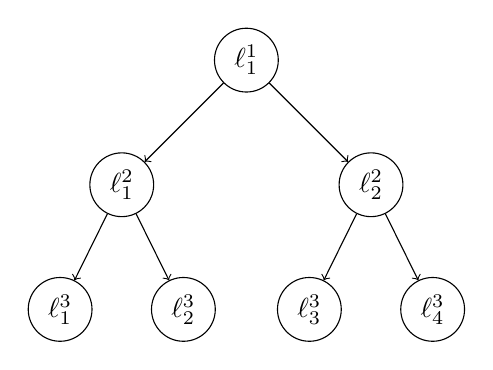
\begin{tikzpicture}[]
\node[circle, draw=black](l11) {$\ell^1_1$};
\node[circle, draw=black, below left = 1cm and 1cm of l11](l21) {$\ell^2_1$};
\node[circle, draw=black, below right = 1cm and 1cm of l11](l22) {$\ell^2_2$};
\node[circle, draw=black, below left = 1cm and 0.2cm of l21](l31) {$\ell^3_1$};
\node[circle, draw=black, below right = 1cm and 0.2cm of l21](l32) {$\ell^3_2$};
\node[circle, draw=black, below left = 1cm and 0.2cm of l22](l33) {$\ell^3_3$};
\node[circle, draw=black, below right = 1cm and 0.2cm of l22](l34) {$\ell^3_4$};
\path[->] (l11) edge (l21);
\path[->] (l11) edge (l22);
\path[->] (l21) edge (l31);
\path[->] (l21) edge (l32);
\path[->] (l22) edge (l33);
\path[->] (l22) edge (l34);
\end{tikzpicture}
\caption{Количество объектов из обучающей выборки, доходящих до каждой из вершин}
\label{tree_objects}
\end{figure}

Нам нужно проверить $d$ признаков по $\ell^i_j - 1$ порогу. Подсчёт метрики качества разбиения занимает $O(\ell^i_j)$ времени. Однако можно реализовать \textit{оптимальный} алгоритм с преподсчитанными статистиками, который для каждого признака сможет вычислить метрику \textit{сразу по всем} $\ell^i_j - 1$ порогам за $O(\ell^i_j)$ времени. Следовательно, для одной вершины требуется $d * O(\ell^i_j) = O(d\ell^i_j)$ времени.

Понятно, что $\ell^1_1 = \ell$, поскольку это самая верхняя вершина. Дальше, для любого $i, j$ верно, что $\ell^i_j = \ell^{i + 1}_{2j - 1} + \ell^{i + 1}_{2j}$ по принципу сохранения стоков-истоков (число объектов, исходящих из одной вершины до её детей, равна числу объектов, входящих в эту вершину). Из этого следует, что в сумме на одном уровне будет всего $\ell$ объектов, $\forall i ~:~ \sum\limits^{2^i}_{j=1} \ell^i_j = \ell$. А значит, на построение одного уровня в решающем дереве нам нужно всего $\sum\limits^{2^i}_{j=1} O(d\ell^i_j) = O(d\ell)$, а уровней всего $D$. Следовательно на построение одного дерева необходимо $T_{tree} = O(Dd\ell)$ времени. У нас $N$ деревьев, следовательно общее время на построение всех деревьев, а значит и на всё обучение: $O(NDd\ell)$

На стадии построения прогноза для объекта $x$ он «пропускается» через дерево от корня к листьям, тем самым проходя путь из не более чем $D$ внутренних вершин, в каждой из которых происходит проверка предиката за константное время. Отсюда имеем асимптотику для построения прогноза композиции — $O(ND)$.

\end{esSolution}

Что будет быстрее~--- бэггинг или бустинг?
Чёткого ответа нет.
С одной стороны, в бустинге используются неглубокие деревья.
Поскольку обучение градиентного бустинга является «направленным», есть шанс,
что ему потребуется меньшее по сравнению со случайным лесом количество базовых алгоритмов для достижения того же качества композиции.
С другой стороны, обучение разных базовых моделей в бэггинге никак не связано, поэтому можно строить все модели параллельно.
В бустинге такого преимущества нет~--- мы не можем обучать~$N$-е дерево, пока не построим все предыдущие.
Как правило, в бустинге распараллеливают только выбор лучших предикатов, но это можно сделать и в бэггинге.

\begin{thebibliography}{1}
\bibitem{lu20accelerating}
    \emph{Lu, Haihao and Karimireddy, Sai Praneeth and Ponomareva, Natalia and Mirrokni, Vahab} (2020).
    Accelerating Gradient Boosting Machines.~//
    Proceedings of the Twenty Third International Conference on Artificial Intelligence and Statistics,
    516--526.
\end{thebibliography}


\end{document}
